\documentclass{article}

\usepackage{caption}
\usepackage{subcaption}
\usepackage{graphicx}
\usepackage{tikz}
\usepackage{tikzsymbols}
\usetikzlibrary{calc,patterns,shapes.geometric}
\usepackage{float}

\def\centerarc[#1](#2)(#3:#4:#5){\draw[#1] ($(#2)+({#5*cos(#3)},{#5*sin(#3)})$) arc (#3:#4:#5);}

\pagestyle{empty}
\begin{document}
	\centering
	\begin{figure}[H]
		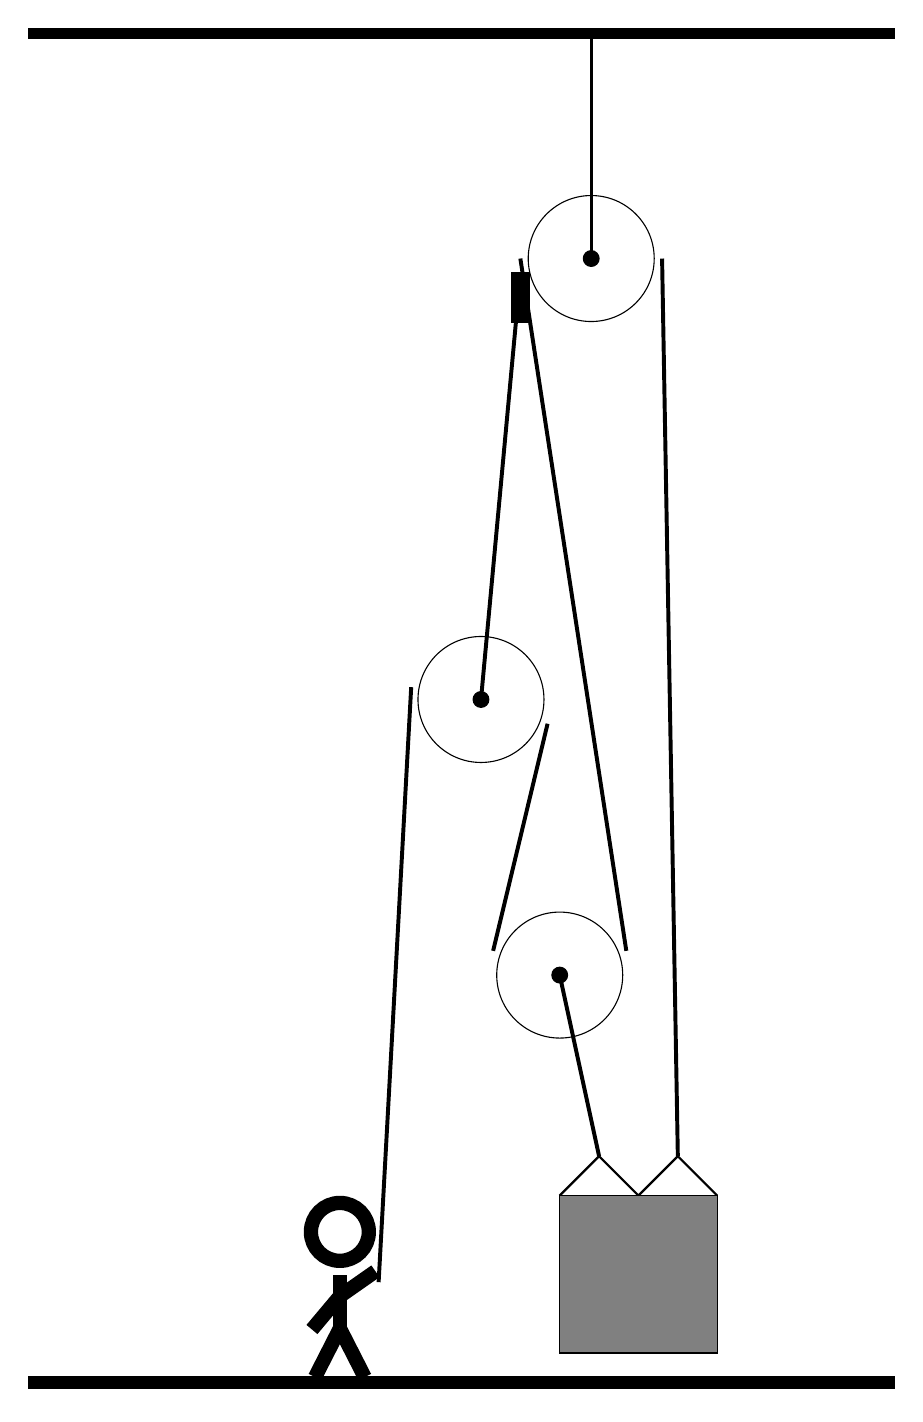
\begin{tikzpicture}
			%%%%% START %%%%%
			\def\a{14}
			\def\radrp{0.9}
			\def\radlg{0.8}
			\def\radsm{0.1}
			\def\xone{-0.25}
			\def\yone{\a -\a*0.6}
			\def\xtwo{0.75}
			\def\ytwo{\a - \a*0.85}
			\def\xthree{\xone+1.4}
			\def\ythree{\a-\a*0.2}
			\def\dx{-2}
			\def\dy{-1.9}
			\def\dw{1.75mm}
			\def\xbox{0.75}
			\def\ybox{\a-\a*1.05}
			\def\width{0.5mm}
			\def\bump{0.3}
			
			\draw[fill=black] (-6,\a) rectangle (5,\a+0.125);
			
			\draw (\xone,\yone) circle (\radlg);
			\draw[fill=black] (\xone,\yone) circle (\radsm);
			
			\draw (\xtwo,\ytwo) circle (\radlg);
			\draw[fill=black] (\xtwo,\ytwo) circle (\radsm);
			
			\draw (\xthree,\ythree) circle (\radlg);
			\draw[fill=black] (\xthree,\ythree) circle (\radsm);
			\draw[very thick] (\xthree,\ythree) -- (\xthree,\a);
			
			\draw[thick]  (\xbox,\ybox) -- (\xbox+0.5,\ybox+0.5) -- (\xbox+1,\ybox) -- (\xbox+1.5,\ybox+0.5) -- (\xbox+2,\ybox);
			\draw[fill=black!50] (\xbox,\ybox) rectangle (\xbox+2,\ybox-2); 
			
			 \draw[line width=\width] (\xone,\yone) -- (\xthree-\radrp,\ythree-0.2);
			 \draw[line width=\width, fill=black](\xthree-\radrp-0.1,\ythree-0.8) rectangle (\xthree-\radrp+0.1,\ythree-0.2); 
			\draw[line width=\width] (\dx+0.45,\dy+0.1) -- ({\xone+\radrp*cos(170)}, {\yone+\radrp*sin(170)});
			\centerarc[line width=\width](\xone,\yone)(-20:170:\radrp);
			\draw[line width=\width] ({\xone+\radrp*cos(20)}, {\yone-\radrp*sin(20)}) -- ({\xtwo+\radrp*cos(200)}, {\ytwo-\radrp*sin(200)});
			\centerarc[line width=\width](\xtwo,\ytwo)(160:380:\radrp);
			\draw[line width=\width] ({\xtwo+\radrp*cos(340)},{\ytwo-\radrp*sin(340)}) -- (\xthree-\radrp,\ythree);
			\draw[line width=\width](\xtwo,\ytwo) -- (\xbox+0.5,\ybox+0.5);
			\centerarc[line width=\width](\xthree,\ythree)(0:180:\radrp);
			\draw[line width=\width] (\xthree+\radrp,\ythree) -- (\xbox+1.5,\ybox+0.5);
			
			\node at (\dx,\dy) {\Strichmaxerl[10][50][35]};
			
			\draw[fill=black] (-6,-3) rectangle (5,-3.15);
			%%%%% END %%%%%
		\end{tikzpicture}
	\end{figure}
	
\end{document}